\documentclass[a4paper,11pt]{article}
\usepackage[T1]{fontenc}				% Para que se puedan formar tildes como una sola letra
\usepackage[utf8]{inputenc}             % Para poder escribir tildes
\usepackage{textcomp}					% M\`as caracteres acentuados
\usepackage{multicol}					% Crea ambientes donde se puede escribir en varias columnas
\usepackage{soul}
\usepackage{mathtools}
\usepackage{amsmath,amssymb,amsfonts,latexsym,cancel}	% Paquete para la creaci\'on de ambientes y s\'imbolos matem\'aticos
\usepackage{amssymb}
\usepackage{multirow}
\usepackage[table,xcdraw]{xcolor}
\usepackage{anysize}
\usepackage{fancyhdr}
\usepackage{xcolor}	
\usepackage{graphicx}	
\usepackage{caption}
\usepackage{adjustbox}
\usepackage[colorlinks=true,backref=true,linkcolor=azul,citecolor=g,urlcolor=azul]{hyperref}
\IfFileExists{enumitem.sty}{\usepackage{enumitem}}{}
\usepackage{floatrow}
%---------------------------------------------------------------------------------------------------------------------------
					% Para ajustar m\'argenes del documento
\marginsize{1cm}{1cm}{0.5cm}{0.3cm}
%\marginsize{L}{R}{U}{D}
\captionsetup{font={scriptsize}}
%\setlength{\captionmargin}{20pt}
%\newcommand{\captionfonts}{\scriptsize}
%\makeatletter  % Allow the use of @ in command names
%\long\def\@makecaption#1#2{%
%  \vskip\abovecaptionskip
%  \sbox\@tempboxa{{\captionfonts #1: #2}}%
%  \ifdim \wd\@tempboxa >\hsize
%    {\captionfonts #1: #2\par}
%  \else
%    \hbox to\hsize{\hfil\box\@tempboxa\hfil}%
%  \fi
 % \vskip\belowcaptionskip}
%\makeatother
%---------------------------------------------------------------------------------------------------------------------------
					% Para editar encabezados y pies de p\'agina
\pagestyle{fancy}
\fancyfoot[C]{}
\fancyhead[r]{}
\fancyhead[l]{}
\fancyhead[c]{}

%---------------------------------------------------------------------------------------------------------------------------
				% Para generar y usar colores
\definecolor{azul}{rgb}{0,0,1}
\definecolor{g}{cmyk}{0.05,0.05,0.05,0.05}
%\definecolor{``nombre''}{``formato''}{0.0,0.0,0.0,0.0}
%---------------------------------------------------------------------------------------------------------------------------
				% Para poder introducir gr\'aficas y fotos en formatos dif. a eps
\DeclareGraphicsExtensions{.pdf,.png,.jpg}
%---------------------------------------------------------------------------------------------------------------------------
% Para insertar v\`inculos e hiperv\`iculos
%linkcolor=color (red) links internos
%citecolor=color (green) color de citaciones
%filecolor=color (magenta) ficheros locales
%pagecolor=color (red) otras p{\'a}ginas
%urlcolor=color (cyan) color de direcciones de internet url externas
%Otras opciones:
%backref=true para a{\~n}adir un link de retorno en la bibliograf{\'i}a .
%pagebackref=true lo mismo que el anterior pero ligado a la p{\'a}gina
%---------------------------------------------------------------------------------------------------------------------------
%---------------------------------------------------------------------------------------------------------------------------
\parindent 0mm						% Indexado o sangrado
%---------------------------------------------------------------------------------------------------------------------------
%T\`iTULO
\makeatletter
\renewcommand{\maketitle}{
\begin{center}
\begin{normalsize}\textbf{\@title}\end{normalsize}\\
\begin{normalsize}\@author\end{normalsize}
\end{center}
}
\title{Álgebra - Pr\'actica 1 - Conjuntos, Relaciones y Funciones} 
\author{}
\date{1-2019}

\pdfinfo{%
  /Title    ()
  /Author   ()
  /Creator  ()
  /Producer ()
  /Subject  ()
  /Keywords ()
}
%-----------------Comandos creados para ayudar---------------
\newcommand{\real}{\mathbb{R}}
\newcommand{\resalta}[1]{\colorbox{g}{$\displaystyle #1$}}
\newlength\dlf
\newcommand\alignedbox[2]{
  % #1 = before alignment
  % #2 = after alignment
  &
  \begingroup
  \settowidth\dlf{$\displaystyle #1$}
  \addtolength\dlf{\fboxsep+\fboxrule}
  \hspace{-\dlf}
  \fcolorbox{g}{g}{$\displaystyle #1 #2$}
  \endgroup
}
\newcommand{\corchetes}[1][*]{
   $\{{#1}\}$
}
\newcommand{\partesde}[1][*]{
    \mathcal{P}({#1})
}
%-------------------------------------------------------------
\begin{document}
\renewcommand{\headrulewidth}{0pt} 			% grosor de la l\'inea de la cabecera
\renewcommand{\tablename}{Tabla}
\renewcommand{\figurename}{Fig.}
\renewcommand{\refname}{Bibliograf\'ia y referencias}
\renewcommand{\contentsname}{Tabla de contenido}
%\renewcommand{\citeform[1]{[#1]}
\maketitle
\section*{Conjuntos}
%Ejercicio 1----------------------
    \begin{enumerate}
        \item Dado el conjunto $A=\{1,2,3\}$, determinar c\'uales de las siguientes afirmaciones son verdaderas:
        \begin{enumerate}[label = \roman*)]
            \item $1\in A$\\
                \colorbox{g}{\textit{Verdadero}}, 1 est\'a el la lista de elementos de $A$.
            \item $\{1\}\subseteq A$\\
                \colorbox{g}{\textit{Verdadero}}, el conjunto $\{1\}$ es subconjunto de $A$.
            \item $\{2,1\}\subseteq A$\\
                \colorbox{g}{\textit{Verdadero}}, en principio, los elementos de un conjunto no estan ordenados, luego $\{2,1\}=\{1,2\}$, y este conjunto es subconjunto de $A$.
            \item $\{1,3\}\in A$\\
                \colorbox{g}{\textit{Falso}}, el conjunto $\{1,3\}$ es \textit{subconjunto} de $A$, m\'as no est\'a en la lista de elementos de $A$.
            \item $\{2\}\in A$\\
                \colorbox{g}{\textit{Falso}}, Ocurre lo mismo que en el caso anterior.
        \end{enumerate}
%Ejercicio 2----------------------
        \item Dado el conjunto $A = \{1,2,\{3\},\{1,2\}\} $, determinar c\'uales de las siguientes afirmaciones son verdaderas:
        \begin{enumerate}[label = \roman*)]
            \item $3\in A$\\
                \colorbox{g}{\textit{Falso}}, El elemento de $A$ es el conjunto $\{3\}$, no el elemento $3$.
            \item $\{3\} \subseteq A$\\
                \colorbox{g}{\textit{Falso}}, el conjunto $\{3\}$ es \textit{un elemento} de $A$, no un subconjunto.
            \item $\{3\} \in A$\\
                \colorbox{g}{\textit{Verdadero}}.
            \item $\{\{3\}\} \subseteq A$\\
                \colorbox{g}{\textit{Verdadero}}, el conjunto de un \'unico elemento $\{\{3\}\}$ es subconjunto de $A$.
            \item $\{1,2\} \in A$\\
                \colorbox{g}{\textit{Verdadero}}.
            \item $\{1,2\} \subseteq A$\\
                \colorbox{g}{\textit{Falso}}, el conjunto $\{1,2\}$ es \textit{un elemento} de $A$.
            \item $\{\{1,2\}\} \subseteq A$\\
                \colorbox{g}{\textit{Verdadero}}, dado que $\{1,2\}$ es un elemento de $A$, el conjunto creado a partir de este \'unico elemento ser\'a subconjunto de $A$.
            \item $\{\{1,2\},3\} \subseteq A$\\
                \colorbox{g}{\textit{Falso}}, el elemento $3$ no pertenece a $A$, por lo tanto cualquier conojunto que tenga a $3$ no puede ser subconjunto de $A$.
            \item $\emptyset \in A$\\
                \colorbox{g}{\textit{Falso}}, el conjunto vacio es \textit{un subconjunto} de $A$.
            \item $\emptyset \subseteq A$\\
                \colorbox{g}{\textit{Verdadero}}
            \item $A\in A$\\
                \colorbox{g}{\textit{Falso}}, Todo conjunto es subconjunto de s\'i mismo\footnote{Aunque es verdad que pueden darse casos en los que por la misma definici\'on del conjunto, este puede ser parte de s\'i mismo, No en este caso.}.
            \item $A\subseteq A$\\
                \colorbox{g}{\textit{Verdadero}}.
        \end{enumerate}
        \newpage
%Ejercicio 3----------------------
        \item Determinar si $A \subseteq B$ en cada uno de los siguientes casos:
        \begin{enumerate}[label = \roman*)]
                \item $A=\{1,2,3\}$, $B=\{5,4,3,2,1\}$\\
                    \colorbox{g}{\textit{Verdadero}}. los elementos 1, 2, 3 pertenecen a los dos conjuntos.
                 \item $A=\{1,2,3\}$, $B=\{1,2,\{3\},-3\}$\\
                    \colorbox{g}{\textit{Falso}}, ya que el elemento tres no hace parte de los elementos de $B$.
                \item $A=\{x\in \mathbb{R} \colon 2<|x|<3\}$, $B=\{x\in \mathbb{R}\colon x^{2}<3\}$\\
                    \colorbox{g}{\textit{Verdadero}}, ya que los intervalos donde $x$ pertenece a $A$ son $(-3,-2)$ y $(2,3)$, mientras que el intevalo donde $x$ pertenece a $B$ es $(-3,3)$
                \item $A=\{\emptyset\}$, $B=\emptyset$\\
                    \colorbox{g}{\textit{Falso}}, ya que $B$ es el conjunto vacio, $B$ es subconjunto propio de cualquier otro subconjunto, m\'as no tiene ning\'un subconjunto propio.
        \end{enumerate}
%Ejercicio 4---------------------
        \item Describir a los siguentes subconjuntos de $\real$ por comprensi\'on mediante \textit{una sola} ecuaci\'on:
        \begin{enumerate}[label = \roman*)]
            \item $\{-3,1,5\}$: 
            Aunque para describir este conjunto por compreni\'on hay varias maneras, una de las m\'as sencillas es expresar estos valores como el conjunto soluci\'on de las raices de un polinomio, asi, se puede describir el conjunto como:
            \begin{equation}
                \notag \resalta{\{x\in \mathbb{R}\colon (x+3)(x-1)(x-5)=0\}}
            \end{equation}
            $(-\infty,2]\cup[7,+\infty)$: Una buena manera de describir este conjunto es llevandolo a una expresi\'on relacionada con un valor absoluto, esto se intuye por la misma descripci\'on ya dada: que $x$ pertenezca a $(-\infty,2]\cup[7,+\infty)$, solo puede ocurrir si:
           \begin{eqnarray*}
             \notag
                x<2&\wedge& x>7\\
                x-(9/2)<2-(9/2)&\wedge& x-(9/2)>7-(9/2)\\
                x -9/2<-5/2&\wedge& x-9/2>5/2
            \end{eqnarray*}
            Basicamente, al restar a los t\'erminos de las desigualdades $9/2$ logramos ``centrar'' los intervalos respecto al origen para ver m\'as claramente c\'omo reescribir el conjunto. Es claro que el conjunto hace referencia a
            \begin{equation}
                \notag\resalta{\{x \in \real \colon |x-9/2|>5/2\}}
            \end{equation}
            \item Describir a los siguentes subconjuntos de $\real$ por comprensi\'on mediante \textit{una sola} ecuaci\'on:\\
            \begin{minipage}[c]{0.3\linewidth}
                \centering
                    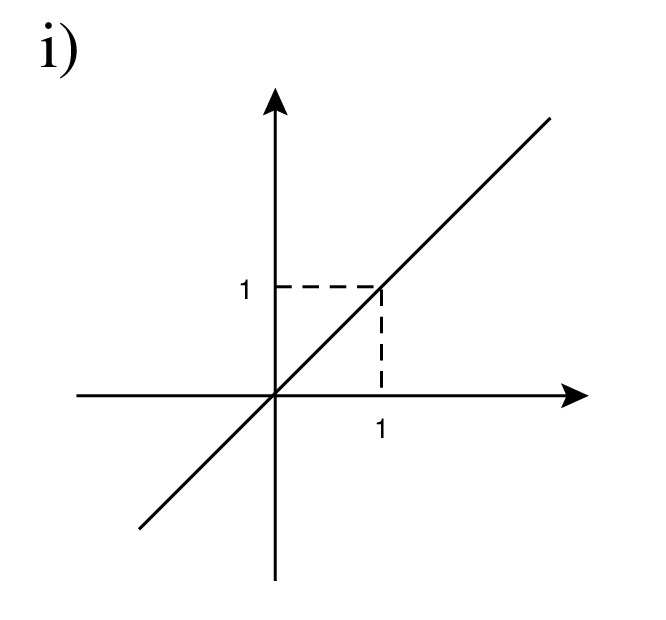
\includegraphics[scale=0.15]{4ii-1}
            \end{minipage}
            \begin{minipage}[c]{0.7\linewidth}
                Esta es la recta $x=y$, por lo tanto la ecuaci\'on que describe este conjunto es
                \begin{equation}
                    \notag \resalta{\{(x,y)\in \real^{2} \colon x=y\}}
                \end{equation}
            \end{minipage}
            \begin{minipage}[c]{0.3\linewidth}
                \centering
                    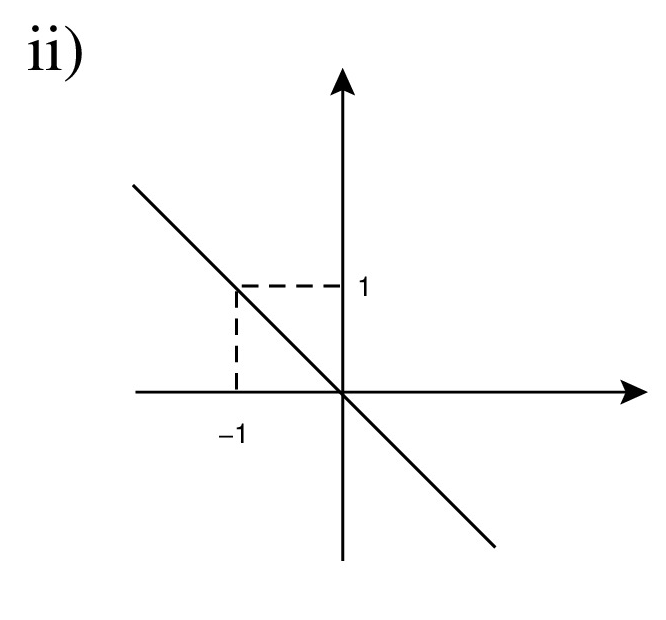
\includegraphics[scale=0.15]{4ii-2}
            \end{minipage}
            \begin{minipage}[c]{0.7\linewidth}
                Esta es la recta $x=-y$, por lo tanto la ecuaci\'on que describe este conjunto es
                \begin{equation}
                    \notag \resalta{\{(x,y)\in \real^{2} \colon x=-y\}}
                \end{equation}
            \end{minipage}
            \begin{minipage}[c]{0.3\linewidth}
                \centering
                    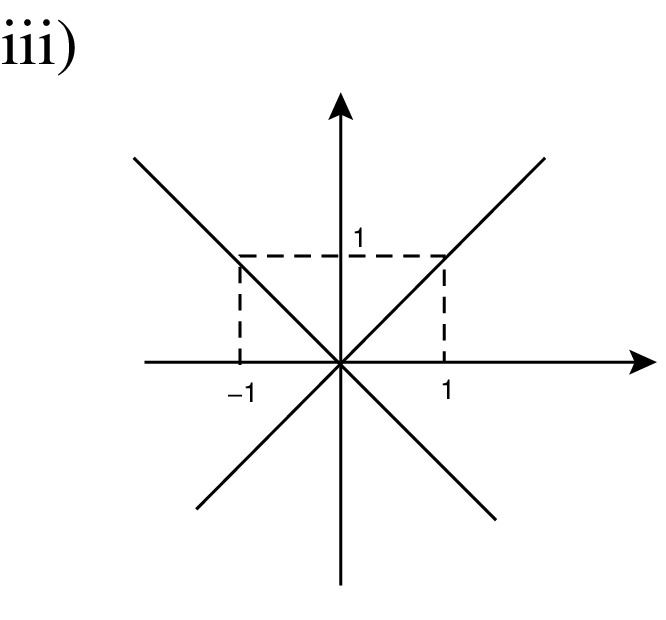
\includegraphics[scale=0.15]{4ii-3}
            \end{minipage}
            \begin{minipage}[c]{0.7\linewidth}
                Este es una conbinaci\'n de los dos grupos anteriores donde tanto $x=y$ como $x=-y$, esto es, que $x=|y|$, y reciprocamente $|x|=y$, luego el conjunto se representa mediante la expresi\'on
                \begin{equation}
                    \notag \resalta{\{(x,y)\in \real^{2} \colon |x|=|y|\}}
                \end{equation}
            \end{minipage}
            \begin{minipage}[c]{0.3\linewidth}
                \centering
                    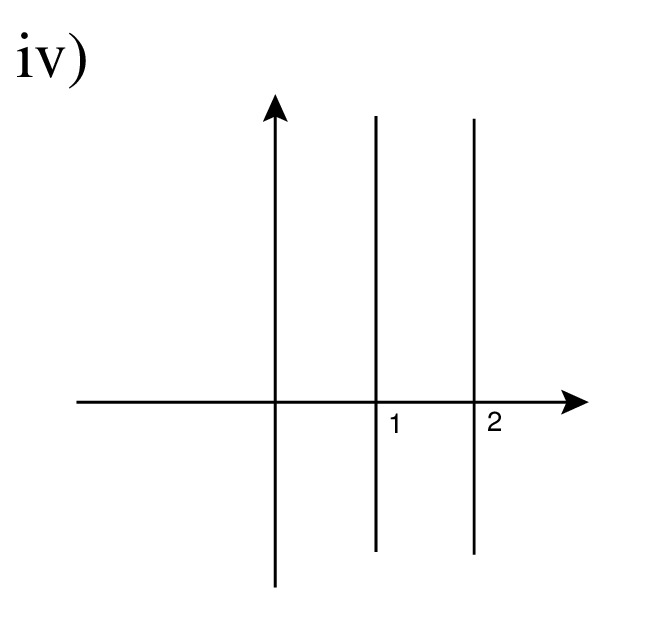
\includegraphics[scale=0.15]{4ii-4}
            \end{minipage}
            \begin{minipage}[c]{0.7\linewidth}
                Aqu\'i se tiene que $x=1$ y $x=2$; una vez m\'as, se puede tomar una expresi\'on para estos dos valores como raices de un polinomio, esto es
                \begin{equation}
                    \notag \resalta{\{(x,y)\in \real^{2} \colon (x-1)(x-2)=0\}}
                \end{equation}
            \end{minipage}
            \begin{minipage}[c]{0.3\linewidth}
                \centering
                    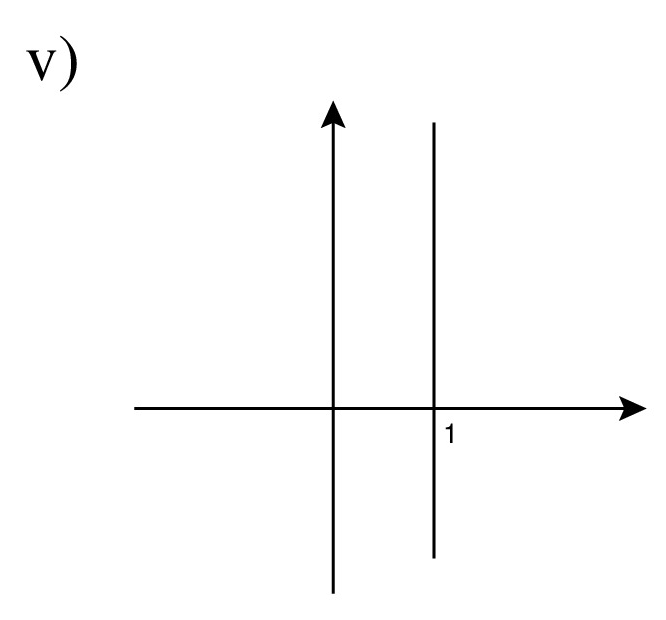
\includegraphics[scale=0.15]{4ii-5}
            \end{minipage}
            \begin{minipage}[c]{0.7\linewidth}
                Nuevamente podemos ver que el valor $x=1$ es la soluci\'on a una ecuaci\'on autoevidente
                \begin{equation}
                    \notag \resalta{\{(x,y)\in \real^{2} \colon x=1\}}
                \end{equation}
            \end{minipage}
            \begin{minipage}[c]{0.3\linewidth}
                \centering
                    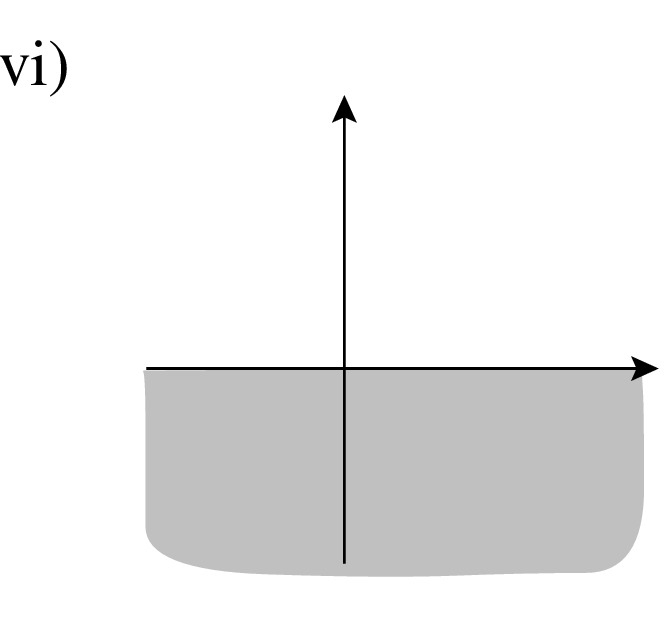
\includegraphics[scale=0.15]{4ii-6}
            \end{minipage}
            \begin{minipage}[c]{0.7\linewidth}
                En este caso la expresi\'on que es m\'as \'util es una desigualdad 
                \begin{equation}
                    \notag \resalta{\{(x,y)\in \real^{2} \colon y\leq 0\}}
                \end{equation}
            \end{minipage}
        \end{enumerate}
%Ejercicio 5---------------------------------------------------------------
        \item Dados los subconjunto $A=\{1,-2,7,3\}$, $B=\{1,\{3\},10\}$ y $C=\{-2,\{1,2,3\},3\}$ del conjunto referencial $V=\{1,\{3\},-2,7,10,\{1,2,3\},3\}$ hallar:
        \begin{enumerate}[label = \roman*)]
            \item $A\cap(B\bigtriangleup C)$\\\\
            La diferencia sim\'etrica entre dos conjuntos dice que se toman los elementos que pertecen a uno u otro de los dos conjuntos, pero no aquellos que pertenezcan simultaneamente a ambos, esto es:
            \begin{align*}
                A\cap(B\bigtriangleup C)) &= A\cap(B\cup C - B\cap C)
                \intertext{Ahora, el conjunto $B\cap C = \emptyset$, por lo que la operaci\'on queda:}
                A\cap(B\bigtriangleup C) &= A\cap(B\cup C)
            \end{align*}
            esto es:
            \begin{equation}
                \notag \resalta{A\cap(B\bigtriangleup C) = \{1,-2,3\}}
            \end{equation}        
            \item $(A\cap B)\bigtriangleup(A\cap C)$\\\\
            Primero se hayan los conjuntos correspondientes a las intersecciones, y luego tomamos su diferencia sim\'etrica, as\'i tenemos que
            \begin{align*}
                (A\cap B)&=\{1\}\\
                (A\cap C)&=\{-2,3\}\\
                \alignedbox{(A\cap B)\bigtriangleup(A\cap C)}{= \{1,-2,3\}}
            \end{align*}
            \item $A^{c}\cap B^{c}\cap C^{c}$\\
            En este caso, lo mejor es primer aplicar las leyes de De Morgan, de esta manera se logra simplificar bastante el c\'alculo del conjunto.
            \newpage
            Aplicando las leyes de De Morgan tenemos:
            \begin{align*}
                A^{c}\cap B^{c}\cap C^{c} &= (A\cup B)^{c}\cap C^{c}\\
                                        &= ((A\cup B)\cup C)^{c}\\
                                        &= (A\cup B\cup C)^{c}
            \end{align*}
            Ahora, al hacer al uni\'on de los conjuntos nos encontramos con
            \begin{align*}
                (A\cup B\cup C) = \{1,-2,7,3,\{3\},10,\{1,2,3\}\}
            \end{align*}
            que es el conjunto referencial $V$, de esta manera tenemos ahora
            \begin{align*}
                A^{c}\cap B^{c}\cap C^{c} &=(A\cup B\cup C)^{c}\\
                                        &=V^{c}\\
                \alignedbox{A^{c}\cap B^{c}\cap C^{c}}{=\emptyset}
            \end{align*}
        \end{enumerate}
%Ejercicio 6-----------------------------------------------------------------------
        \item Dados los subconjuntos $A$, $B$, $C$ de un conjunto referencial $V$, describir $(A\cup B\cup C)^{c}$ en t\'erminos de intersecciones y complementos, y $(A\cap B\cap C)^{c}$ en t\'erminos de uniones y complementos.\\\\
        Simplemente aplicamos las leyes de De Morgan las veces que hagan falta para llegar un resultado en los t\'erminos requeridos, as\'i:\\
        \begin{minipage}[c]{0.5\linewidth}
            \begin{align*}
                (A\cup B\cup C)^{c} &= ((A\cup B)\cup C)^{c}\\
                                    &= (A\cup B)^{c}\cap C^{c}\\
                \alignedbox{(A\cup B\cup C)^{c}}{=A^{c}\cap B^{c}\cap C^{c}}
            \end{align*}
        \end{minipage}
        \begin{minipage}[c]{0.5\linewidth}
            \begin{align*}
                (A\cap B\cap C)^{c} &= ((A\cap B)\cap C)^{c}\\
                                    &= (A\cap B)^{c}\cup C^{c}\\
                \alignedbox{(A\cap B\cap C)^{c}}{=A^{c}\cup B^{c}\cup C^{c}}
            \end{align*}
        \end{minipage}
%Ejercicio 7-------------------------------------------------------------------
        \item Sean $A$, $B$ y $C$ conjuntos. Representar en un diagrama de Venn\\
        \begin{enumerate}[label = \roman*)]
            \begin{minipage}[c]{0.3\linewidth}
                \item $(A\cup B^{c})\cap C$\\\\
                \centering
                    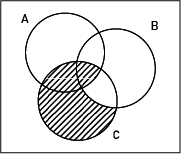
\includegraphics[scale=0.6]{7-i}
            \end{minipage}
            \begin{minipage}[c]{0.3\linewidth}
                \item $A\bigtriangleup(B\cup C)$\\\\
                \centering
                    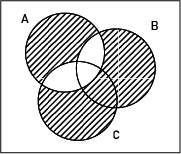
\includegraphics[scale=0.6]{7-ii}
            \end{minipage}
            \begin{minipage}[c]{0.3\linewidth}
                \item $A\cup (B\bigtriangleup C)$\\\\
                \centering
                    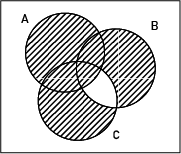
\includegraphics[scale=0.6]{7-iii}
            \end{minipage}
        \end{enumerate}
%Ejercicio 8 -----------------------------------------------------------------------------------
        \item Encontrar f\'ormulas que describan las partes rayadas de los siguentes diagramas de Venn, utilizando \'unicamente intersecciones, uniones y complementos.\\
        \begin{enumerate}[label = \roman*)]
            \begin{minipage}[t]{0.5\linewidth}
                \item
                \begin{center}
                    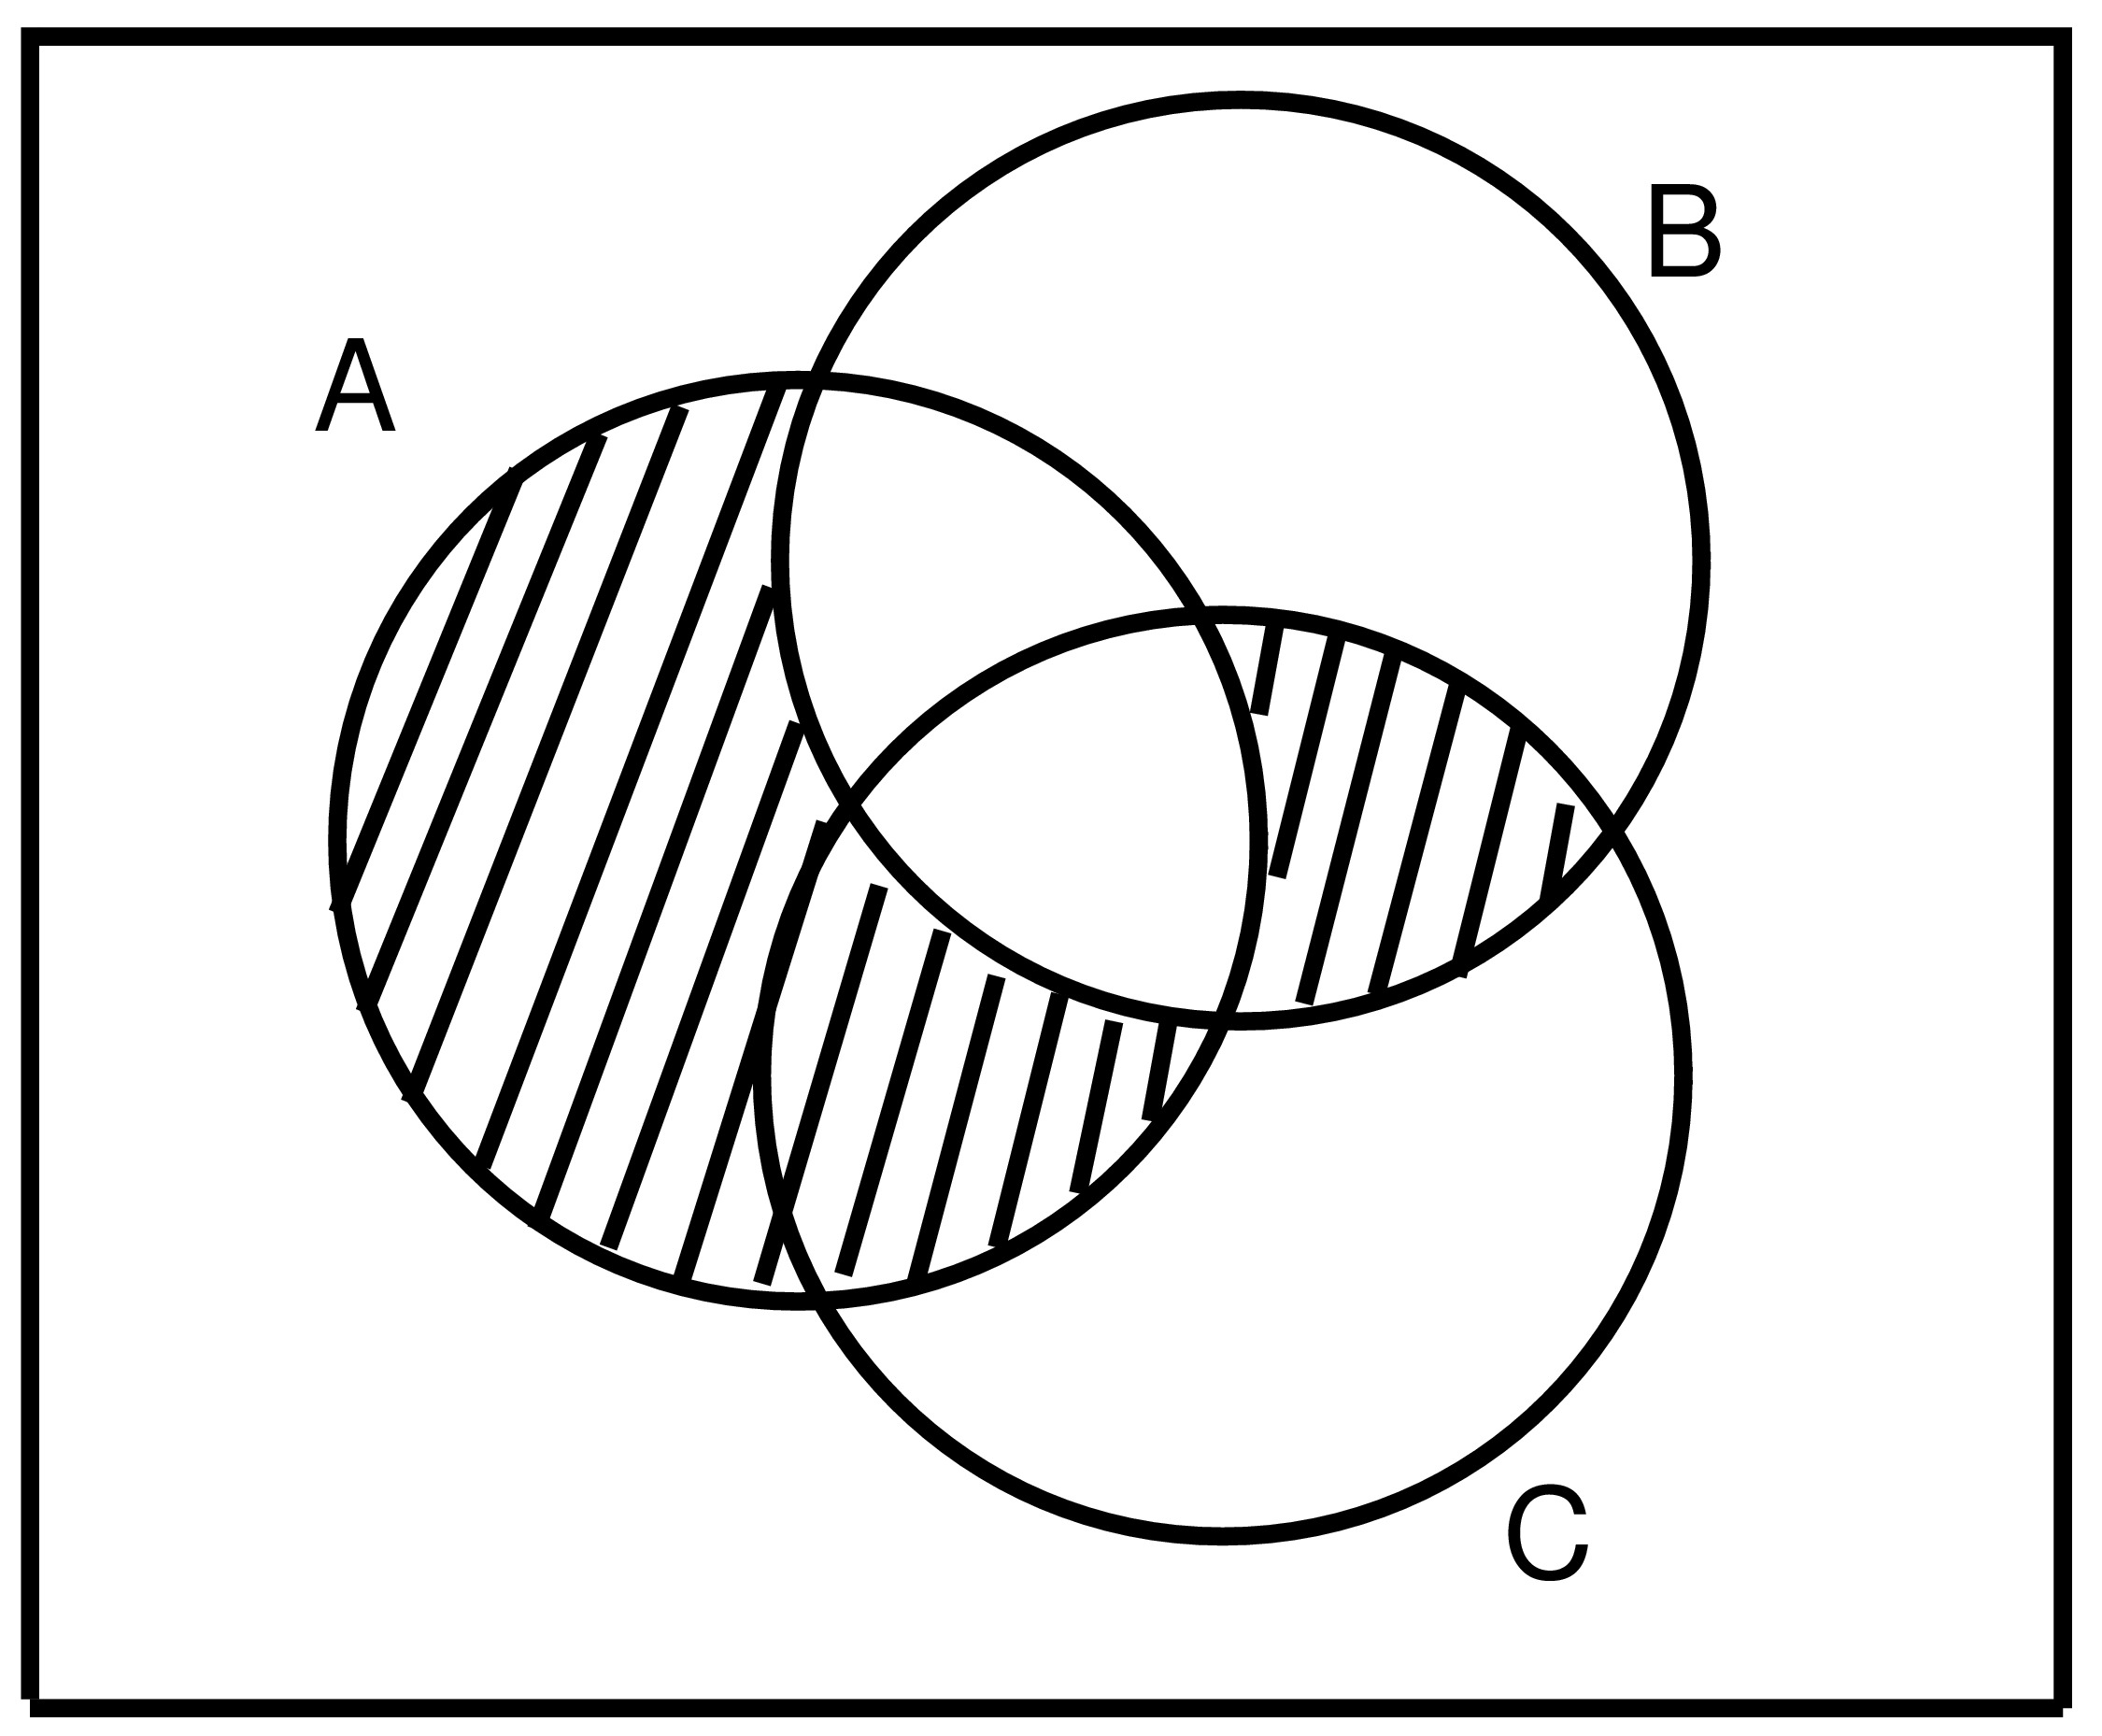
\includegraphics[scale=0.05]{8-i}\\
                \end{center} 
                {\footnotesize 
                    \begin{align*}
                        R &= (A-B)\cup ((B\cap C)-A)\\
                        \alignedbox{R}{=(A-B)\cup (B\cap C)\cap A^{c})}
                    \end{align*}
                }
            \end{minipage}
            \begin{minipage}[t]{0.5\linewidth}
                \item
                \begin{center}
                    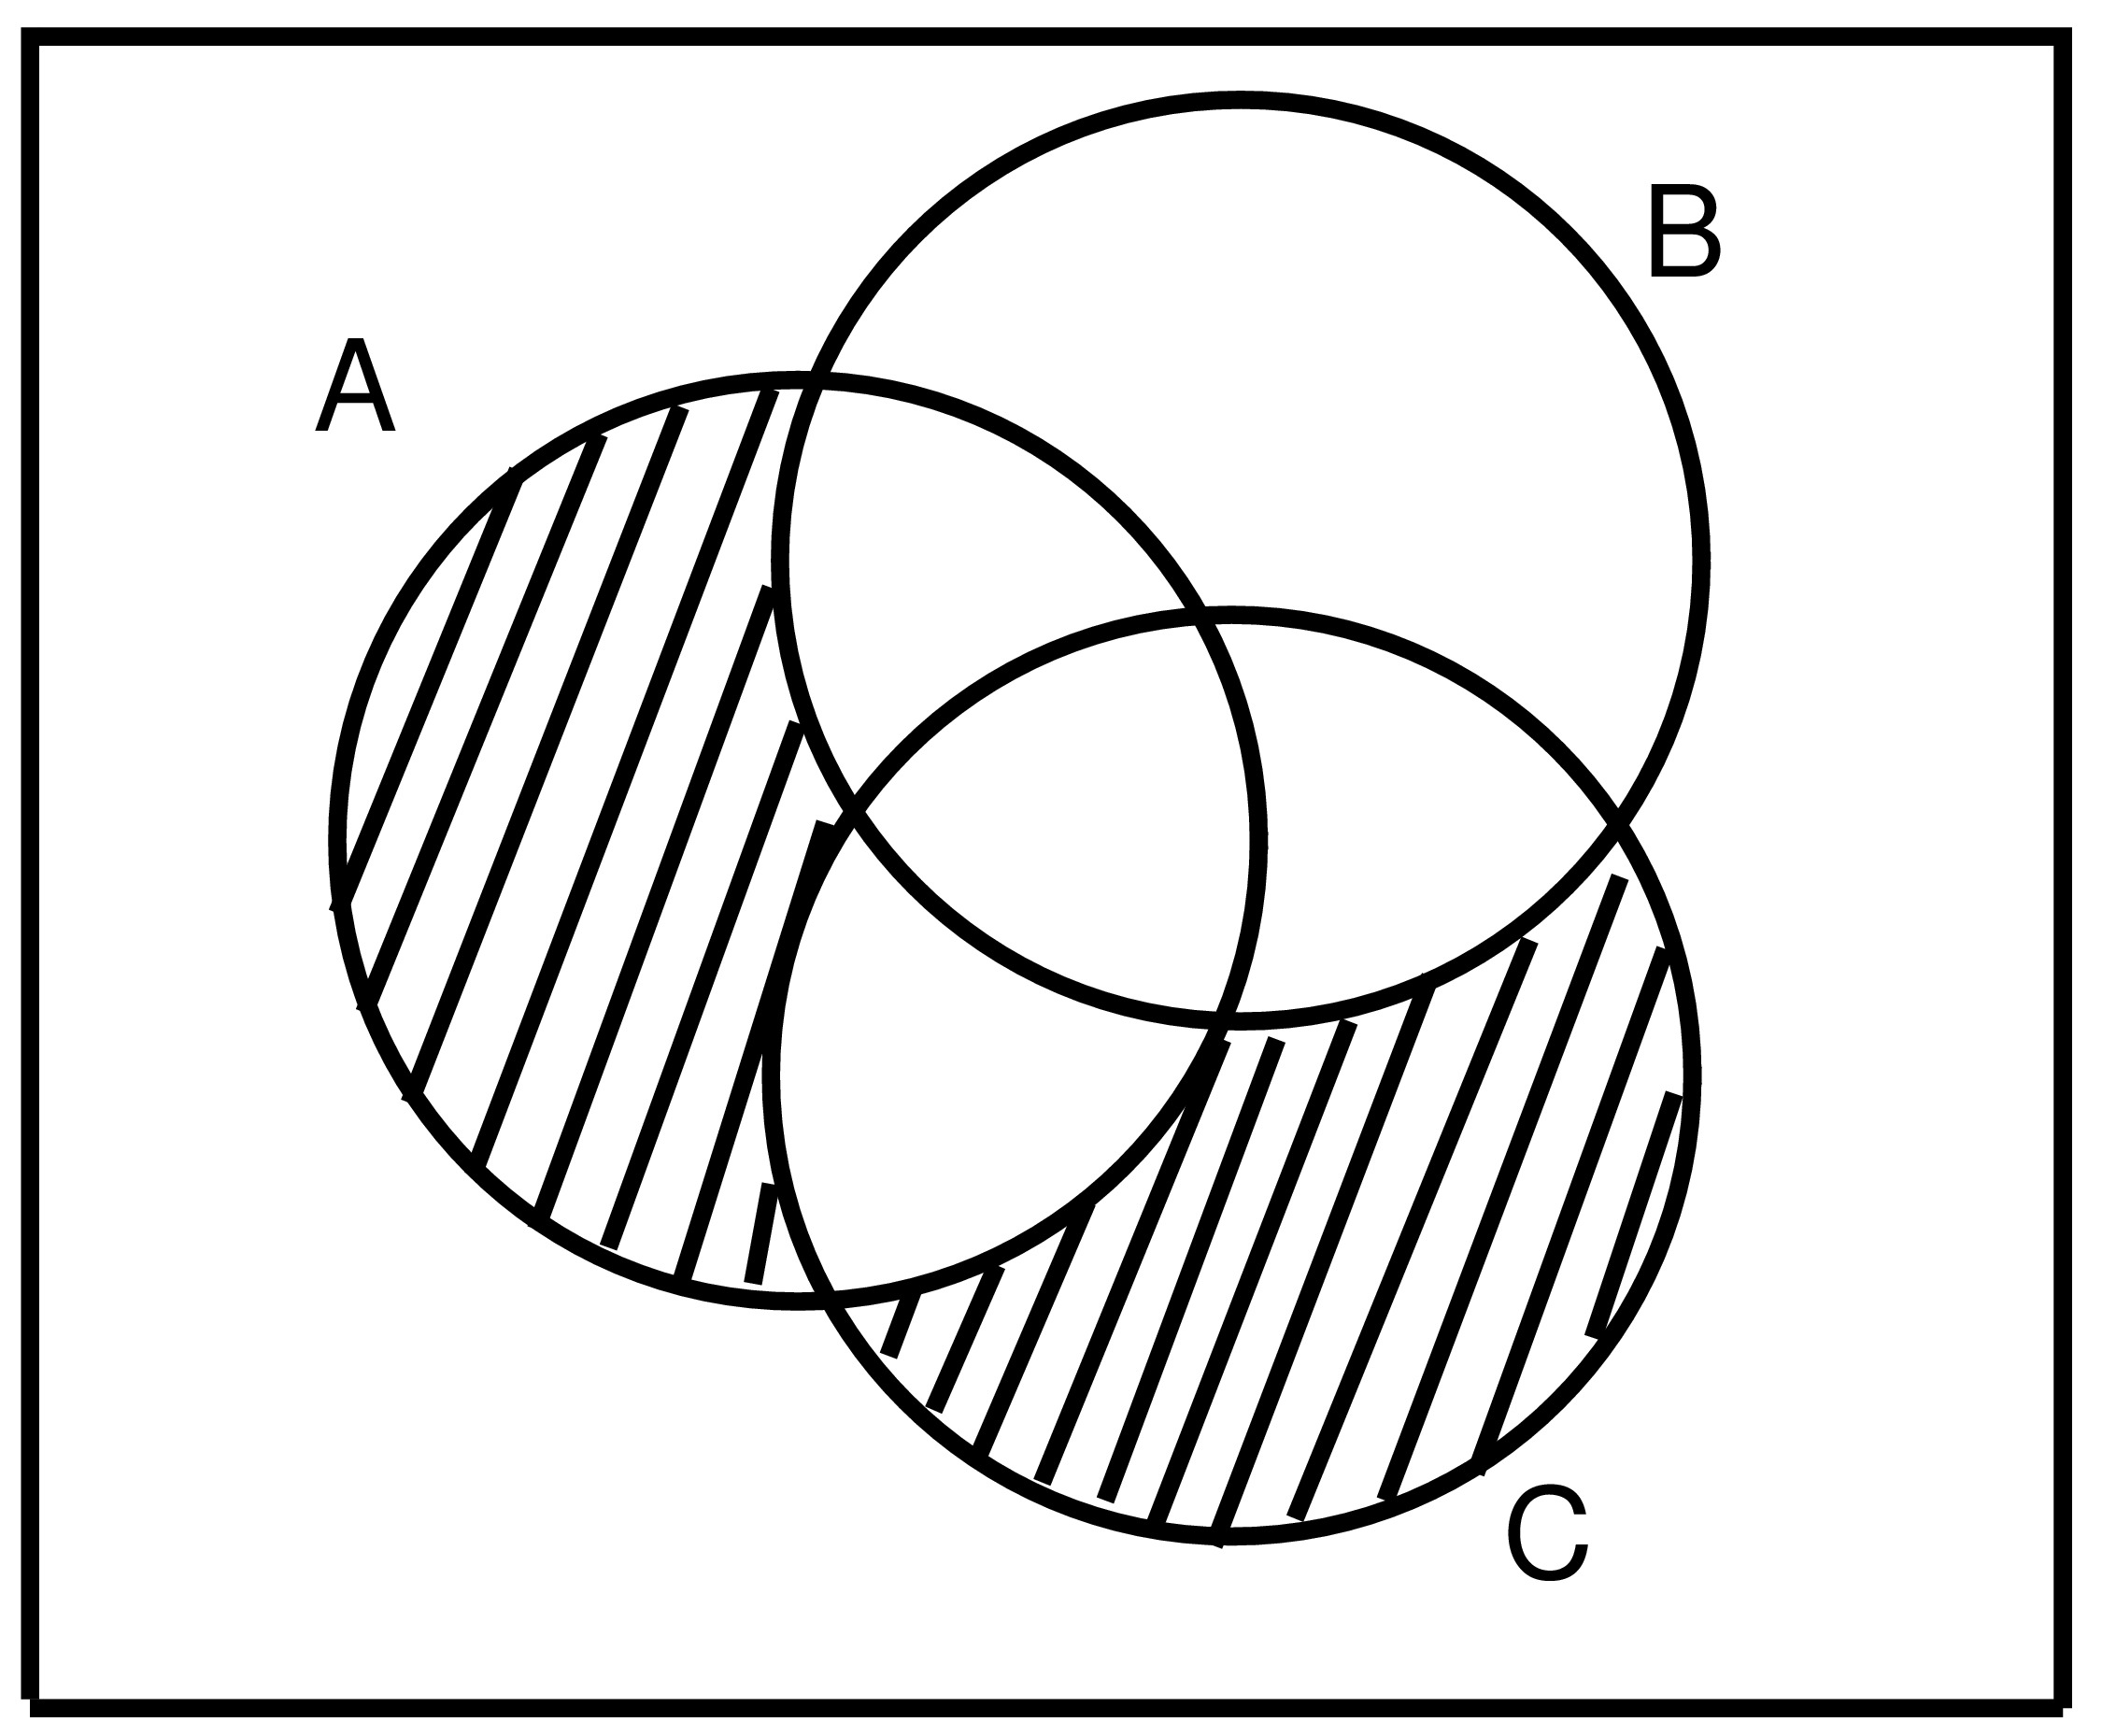
\includegraphics[scale=0.05]{8-ii}\\
                \end{center} 
                {\footnotesize
                    \begin{align*}
                        R &= ((A-B)\cup(C-B))-(A\cap C)\\
                        &= ((A\cap B^{c})\cup(C\cap B^{c}))\cap(A\cap C)^{c})\\
                        \alignedbox{R}{=((A\cup C)\cap B^{c})\cap (A\cap B)^{c}}
                    \end{align*}
                }
            \end{minipage}
            \newpage
            \begin{minipage}[t]{0.3\linewidth}
                \item
                \begin{center}
                    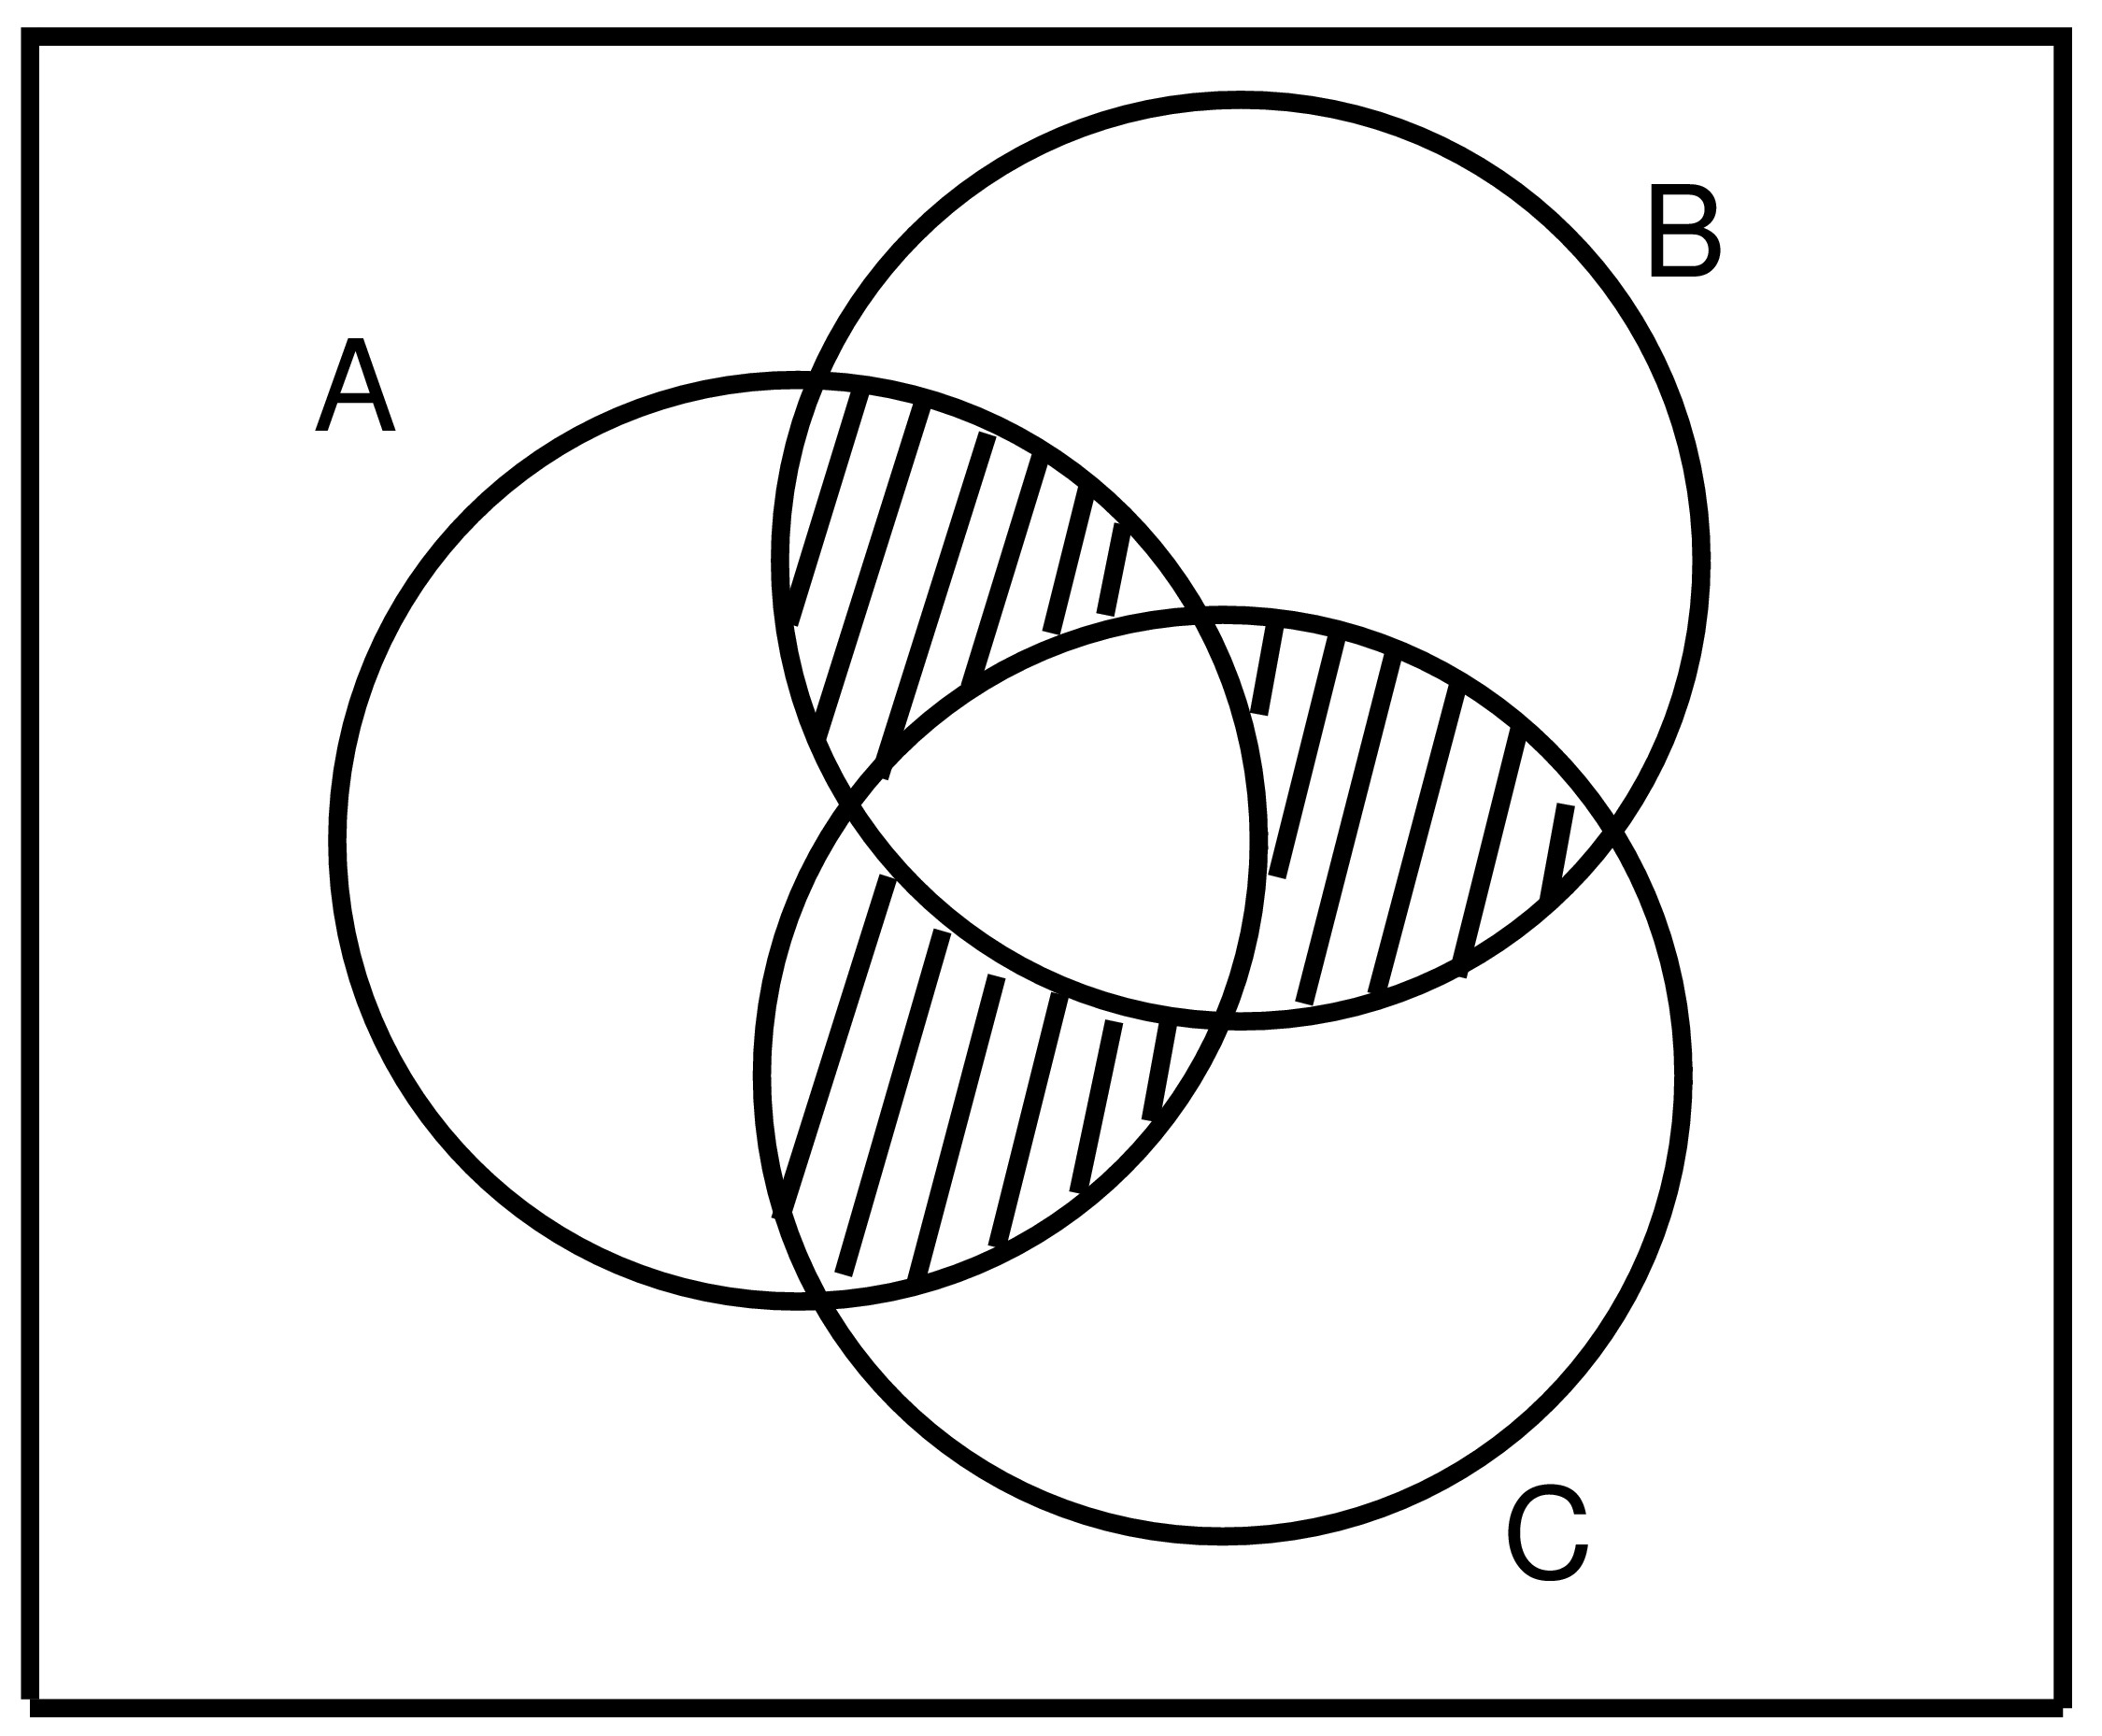
\includegraphics[scale=0.05]{8-iii}\\
                \end{center} 
            \end{minipage}
            \begin{minipage}[t]{0.7\linewidth}
                {\footnotesize
                    \begin{align*}
                        R &= ((A\cap B)\cup(A\cap C)\cup(B\cap C))-((A\cap B)\cap(A\cap C)\cap(B\cap C))\\
                        &= ((A\cap B)\cup(A\cap C)\cup(B\cap C))\cap ((A\cap B)\cap(A\cap C)\cap(B\cap C))^{c}\\
                        &= ((A\cap B)\cup(A\cap C)\cup(B\cap C))\cap ((A\cap B)^{c}\cup(A\cap C)^{c}\cup(B\cap C)^{c})\\
                        &= ((A\cap B)\cup(A\cap C)\cup(B\cap C))\cap ((A^{c}\cup B^{c})\cup(A^{c}\cup C^{c})\cup(B^{c}\cup C^{c}))\\
                        \alignedbox{R}{= ((A\cap B)\cup(A\cap C)\cup(B\cap C))\cap(A^{c}\cup B^{c}\cup C^{c})}
                    \end{align*}
                }
            \end{minipage}
        \end{enumerate}
%Ejercicio 10 ------------------------------------------------------------------
        \item Hallar el conjunto $\mathcal{P}(A)$ (Partes de $A$)\footnote{Partes de $A$ se define como en conjunto de todos los subconjunto de $A$.} en los casos
        \begin{enumerate}[label = \roman*)]
            % i)----------------------------------
            \begin{minipage}[c]{0.2\linewidth}
                \item $A=\{1\}$
            \end{minipage}
            \begin{minipage}[c]{0.8\linewidth}
                \resalta{\mathcal{P}(A)=\{\emptyset ,\{1\}\}}
            \end{minipage}
            % ii)-------------------------------------
            \begin{minipage}[c]{0.2\linewidth}
                \item $A=\{a,b\}$
            \end{minipage}
            \begin{minipage}[c]{0.8\linewidth}
                \resalta{\mathcal{P}(A)=\{\emptyset ,\{a\},\{b\},\{a,b\}\}}
            \end{minipage}
            %iii)------------------------------
            \begin{minipage}[c]{0.2\linewidth}
                \item $A=\{1,\{1,2\},3\}$
            \end{minipage}
            \begin{minipage}[c]{0.8\linewidth}
                \resalta{\mathcal{P}(A)=\{\corchetes[1],\corchetes[\{1,2\}], \corchetes[3],
                \corchetes[1,\{1,2\}],\corchetes[\{1,2\},3],\corchetes[1,3],\corchetes[1,\{1,2\},3]\}}
            \end{minipage}
        \end{enumerate}
%Ejercicio 10 -------------------------------------       
        \item Sean $A$ y $B$ conjuntos. Probar que $\mathcal{P}(A)\subseteq \mathcal{P}(B)\Leftrightarrow A \subseteq B$
        \begin{itemize}
            \item[$\Rightarrow$] $\mathcal{P}(A)\subseteq \mathcal{P}(B)\Rightarrow A \subseteq B$\\\\
            Si $\partesde[A]$ es subconjunto de $\partesde[B]$, dado que $A\in\partesde[A]$, $A$ pertenecerá obviamente a $\partesde[B]$, luego, por la definición del conjunto de partes, se debe tener que $A\subseteq B$.\\
            \item[$\Leftarrow$] $A \subseteq B \Rightarrow \mathcal{P}(A)\subseteq \mathcal{P}(B) $\\\\
            Supongamos que  $A\subseteq B$ pero $\partesde[A] \not\subseteq \partesde[B]$, entonces debería existir un subconjunto de $A$ que no es ninguno de los subconjuntos de $B$, lo que implicaría que al menos un elemento $x$, que cumple $x\in A$ no pertenece a $B$, pero entonces, si $x\in A$ y $x\not\in B$, no puede ser que $A\not\subseteq B$, que contradice nuestra suposición inicial. $\blacksquare$
        \end{itemize}
%Ejercicio 11 -------------------------------------
        \item Sean $p$ y $q$ proposiciones verdaderas o Falsas. Comparar las tablas de verdad de
        \begin{center}
            $p\Rightarrow q$, \hspace*{12pt} $\sim q \Rightarrow \sim p $, \hspace*{12pt} $\sim p \vee q$, \hspace*{12pt} $\sim(p\wedge q)$\\\vspace{12pt}
            
            \begin{table}[!h]
                \captionsetup{width=.6\textwidth}
                \centering
                    \begin{tabular}{cc|c|c|c|c|c|c|c|c|c}\hline
                        \cellcolor{g} $p$ & \cellcolor{g} $q$   & \cellcolor{g}$p\Rightarrow q$ & \multicolumn{3}{c|}{ \cellcolor{g} $\sim q \Rightarrow \sim p $}  & \multicolumn{2}{c|}{ \cellcolor{g}$\sim p \vee q $}   & \multicolumn{3}{c}{ \cellcolor{g}$\sim(p\wedge \sim q)$} \\
                        \cline{3-11}
                        \multicolumn{2}{c|}{\cellcolor{g}}      & $\Rightarrow$                 & $\sim q$  & $\Rightarrow$     & $\sim p$                          & $\sim p$  & $\vee$                                    & $\sim $   & $\wedge$ & $\sim q$\\\hline
                        V   & V                                 & \cellcolor{g} V               & F         & \cellcolor{g} V   & F                                 & F         & \cellcolor{g} V                           & \cellcolor{g} V         & F        & F      \\%\hline
                        V   & F                                 & \cellcolor{g} F               & V         & \cellcolor{g} F   & F                                 & F         & \cellcolor{g} F                           & \cellcolor{g} F         & V        & V      \\%\hline
                        F   & V                                 & \cellcolor{g} V               & F         & \cellcolor{g} V   & V                                 & V         & \cellcolor{g} V                           & \cellcolor{g} V         & F        & F      \\%\hline
                        F   & F                                 & \cellcolor{g} V               & V         & \cellcolor{g} V   & V                                 & V         & \cellcolor{g} V                           & \cellcolor{g} V         & F        & V      \\\hline     
                    \end{tabular}
                    \caption{Las columnas sombreadas correspondes a los valores de verdad de las expresiones. Como se puede notar, el que tengan los mismos valores implica que son equivalentes.}
                \end{table}
            
        \end{center}
%Ejercicio 12--------------------------------------
        \item Decidir si son verdaderas o falsas.
    \end{enumerate}
\end{document}
